\chapter{Die Eulersche $\phi$-Funktion}\filevideo{Eulersche $\phi$-Funktion}

\section*{Ordnungen und Primitivwurzeln}

\begin{frage*}
	Sei $M \geq 2$. Wie viele invertierbaren Restklassen gibt es modulo $M$?
\end{frage*}

\begin{notat*}
	Wir schreiben
	\[ \phi(M) = |(\Z/M\Z)^*| = |\{0 < a \leq M \mid \ggt(a,M) = 1\}|. \]
\end{notat*}

\begin{exmp*}
	\begin{enumerate}[label={\roman*})]
		\item $\phi(2) = 1, \phi(3)=2, \phi(4)=2, \phi(5)=4, \phi(6)=2$\\
		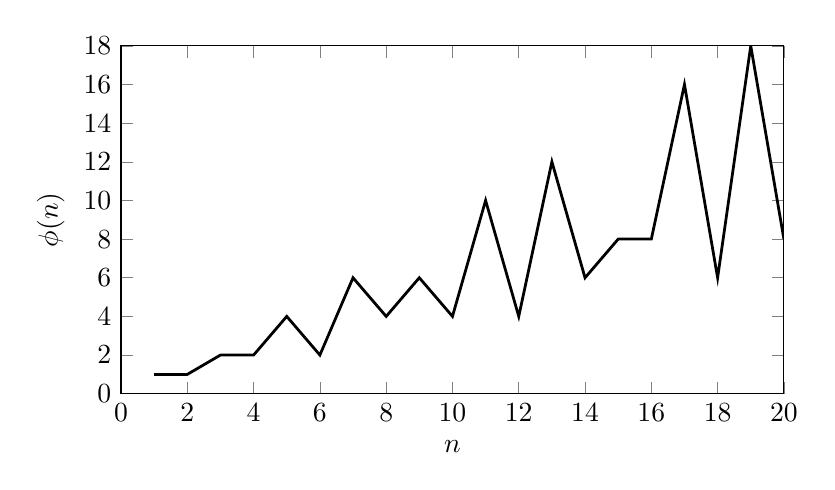
\begin{tikzpicture}
			\begin{axis}
				[
				xlabel={$n$}, ylabel={$\phi(n)$}, xmin=0, xmax=20,
				ymin=0, ymax=18,
				height=6cm,
				width=10cm,
				xtick={0,2,4,6,8,10,12,14,16,18,20},
				ytick={0,2,4,6,8,10,12,14,16,18},
				]
				
				\addplot[line width=1pt]
				coordinates{
					(1,1) (2,1) (3,2) (4,2) (5,4) (6,2) (7,6) (8,4) (9,6) (10,4) (11,10) (12,4) (13,12) (14,6) (15,8) (16,8) (17,16) (18,6) (19,18) (20,8)};
			\end{axis}
		\end{tikzpicture}
		\item Sei $p$ eine Primzahl. Dann ist $\phi(p) = p-1$.
		\item Sei $k \geq 1$ und $p$ prim. Dann gilt
			\begin{align*}
				\phi(p^k) &= p^k - \left|\left\{0 < a \leq p^k \mid \ggt\left(a,p^k\right)>1\right\}\right|\\
				&= p^k - p^{k-1}
			\end{align*}
			Eine Beobachtung:
			\begin{align*}
				\phi(1) + \phi(p) + \phi(p^2) + \dots + \phi(p^k) &= 1 + (p-1) + (p^2-p) + \dots + (p^k-k^{k-1}) \\
				&= p^k
			\end{align*}
	\end{enumerate}
\end{exmp*}

\begin{thm}\autolabel
	Sei $n \in \Z$. Dann gilt
	\[ \sum_{d \mid n} \phi(d) = n. \]
\end{thm}

Nun wollen wir uns mit der Berechnung der Eulerschen $\phi$-Funktion beschäftigen. Für Primzahlpotenzen haben wir das schon getan und wollen dies jetzt auf allgemeine natürliche Zahlen anhand ihrer Primfaktorzerlegung fortsetzen.

\begin{thm}\autolabel\video
	$\phi$ ist eine multiplikative Funktion, d.h. für $m,n \in \N$ mit $\ggt(m,n) = 1$ gilt $$\phi(mn) = \phi(m)\phi(n).$$
\end{thm}

\begin{cor}
	Sei $m = p_1^{k_1} p_2^{k_2} \dotsm p_r^{k_r}$ mit $p_1 < p_1 < \dots < p_r$ Primzahlen und $k_i \geq 0$ für $1 \leq i \leq r$. Dann gilt
	\begin{align*}
		\phi(m) &= \prod_{i=1}^r \left( p_i^{k_1} - p_i^{k_i-1} \right)\\
		\noalign{\centering oder}
		\phi(m) &= m \cdot \prod_{\substack{p \mid  m \\ p \ \text{prim}}} \left( 1-\frac{1}{p} \right).
	\end{align*}
\end{cor}